%%%%% TITLE OF MAIN DOCUMENT %%%%%
%% NUMBER AND TITLE OF SECTION %%


%Some sample text to be displayed above the first subsection

%\subsection{Prinzip}

%Ein Zyklotron besteht aus Zwei hohlen, halbzylindrischen und Duanden an denen eine Spannung mit unterschiedlichem Vorzeichen anliegt, und darüber bzw. darunter liegende Magneten, die ein homogenes Magnetfeld erzeugen. Zudem gibt es einen Einlass und einen Auslass für Teilchen.

%\begin{wrapfigure}{r}{0.4\textwidth} \label{Zyklo}
%
%	\vspace{-10pt}
%	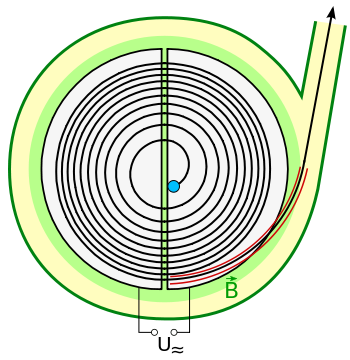
\includegraphics[width=0.35\textwidth]{Zyklotron_Prinzipskizze02.png}
%	\vspace{-13pt}
%	\caption{Prinzipskizze eines Zyklotrons}
%	\vspace{-5pt}	
%	
%\end{wrapfigure}

%\subsubsection{Anwendung}

% Some Formula:

%\begin{equation}
%	x= \frac{y \cdot 13 \pi z}
%			{\cos \alpha}
%\end{equation}

%%%%%%%%%%%%%%%%%%%%%%%
% Eigentlicher Beginn %
%%%%%%%%%%%%%%%%%%%%%%%

\subsection{Abschirmung}
%Cue for a picture
In einem zweidimensionalen elektrischen Feld kann durch einen geschlossenen Ring als Metall ein elektrischen Feld abgeschirmt werden. Dies passiert, da die beweglichen negativen Ladungen im Metall zur einen Seite wandern (entgegen der Feldlinien) und auf der anderen Seite des Ringes ein positive Ladung hinterlassen. Diese Ladungstrennung führt ihrerseits zum Aufbau eines elektrischen Feldes, welches in die entgegengesetzte Richtung zeigt und das \glqq äußere\grqq{} Feld im inneren des Rings neutralisiert. 

Im dreidimensionalen Raum ist dafür eine Hülle nötig, die man dann \glqq Faradayischer Käfig\grqq{} nennt.